\chapter{Proofs and Demonstrations}

\section{Addition over Elliptic Curves and The Group Law}

\hspace{10mm} To construct a suitable notion of addition of points of elliptic curves, let us consider the curve:
\begin{equation}
    E(\R)=\{(x,y) \in \R^2 | y^2=x^3+ax+b; a,b \in \R\} \cup \{\mathcal{O}\}
\end{equation}

\begin{definition}
Let $E(\R)$ be an elliptic curve over the reals and let $P,Q \in E(\R)$. We define $+$ as follows:
\begin{itemize}
    \item If $P=\mathcal{O}$, then $-P=\mathcal{O}$ and $P+Q=Q$. That is, $\mathcal{O}=-\mathcal{O}$ and $\mathcal{O}+Q=Q$.
    
    \item Let $P=(x,y) \in E(\R)$ then $-P=(x,-y) \in E(\R)$.
    
    \item If $P \neq Q$, then take $l=\overline{PQ}$ to be the line that cuts $E(\R)$ at $P$, $Q$, and another point $R$.Then $P+Q=-R$.
\end{itemize}
\end{definition}

\begin{figure}
    \centering
    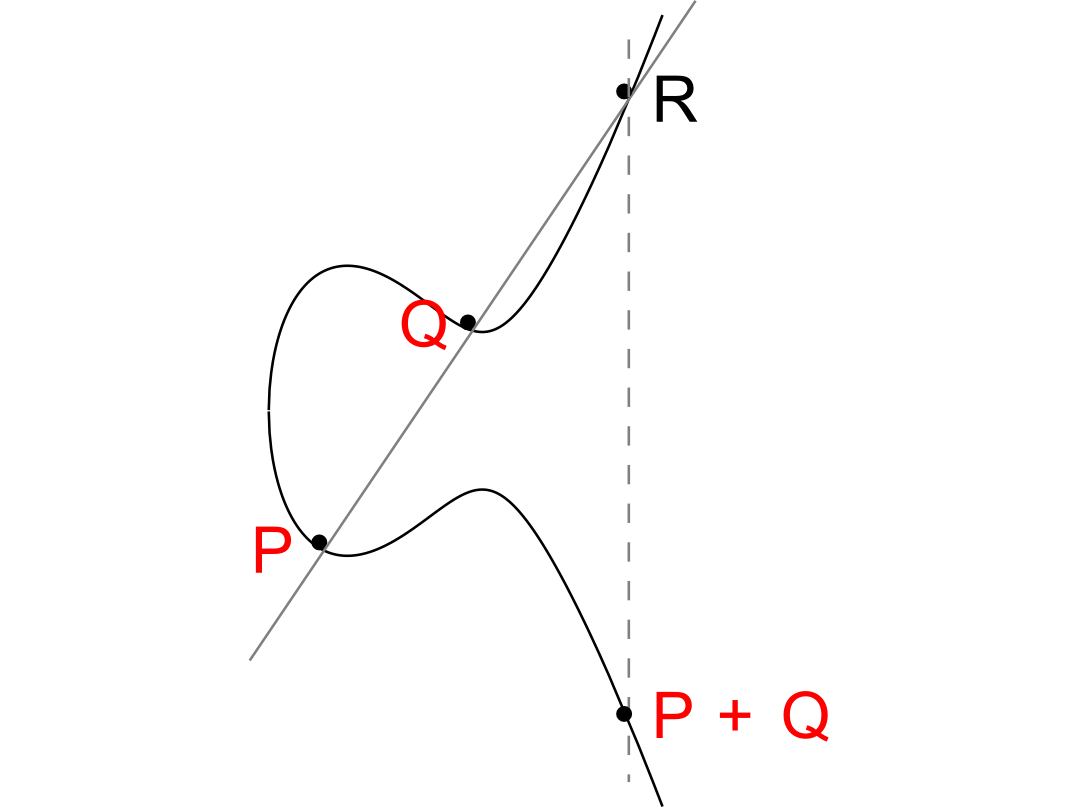
\includegraphics{Figures/EllipticCurveAddition.jpg}
    \caption{Addition of points on an elliptic curve}
    \label{fig:my_label}
\end{figure}

If we let the line $l=\overline{PQ}$ be the plane line $y=\alpha x+\beta$ and $P=(x_1,y_1)$, and $Q=(x_2,y_2)$ be points on $E(\R)$, then we can find the coordinates of $P+Q$ adhering to two cases, the first looks at when $P$ and $Q$ are distinct points, in this case we draw the line that cuts $E(\R)$ at $P$ and $Q$ then we note that $\alpha=\frac{y_2-y_1}{x_2-x_1}$. The latter, concerns itself when $P$ and $Q$ are the same, then it results that the line $y=\alpha x+\beta$ is tangent to the curve, and we consider the derivative of the curve $2y\frac{dy}{dx}=3x^2+a$, and here, $\alpha=\frac{dy}{dx}$, In both cases, $\beta=y_1-\alpha x_1$.

\underline{\keyword{Case 1}} If $P \neq Q$ then $P+Q=(x_3,y_3)$ such that
\begin{equation}
    x_3=(\frac{y_2-y_1}{x_2-x_1})^2-x_1-x_2, y_3=(\frac{y_2-y_1}{x_2-x_1})(x_1-x_1)-y_1
\end{equation}

\underline{\keyword{Case 2}} If $P=Q$ then $P+Q=P+P=(x_3,y_3)$ such that
\begin{equation}
    x_3=(\frac{3x_1^2+a}{2y_1})^2-2x_1, y_3=(\frac{3x_1^2+a}{2y_1})(x_1-x_3)-y_1
\end{equation}

Now that we have found equations for coordinates the point $P+Q$ in $E(\R)$, we can take them to be the coordinates for points on a general elliptic curve $E(K)$.

\hspace{10mm}It can be shown that the elliptic curve $E(K)$ forms an abelian group over $+$, that is for $P,Q,R \in E(K)$:
\begin{itemize}
    \item $P+Q \in E(K)$ (\textit{Closure})
    \item $(P+Q)+R=P+(Q+R)$ (\textit{Associative})
    \item $\exists I \in E(K)$ such that $P+I=I+P=P$ (\textit{Identity Law})
    \item $\exists P^{-1} \in E(K),  \forall P \in E(K)$ such that $P+P^{-1}=P^{-1}+P=I$ (\textit{Inverse Law})
    \item $P+Q=Q+P$ (\textit{Commutative})
\end{itemize}
In fact, it follows by our definition of $+$ over $E(K)$ that commutativity, and the identity and inverse laws are satisfied, where $I=\mathcal{O}$ and $P^{-1}=-P$, it is also rather easy to show closure. Thus, the only law left to prove, is associativity, but the proof for it is beyond the scope of this paper, so we simply accept it as true. In fact, we will go on to prove associativity in a much simpler case in the next section, rather than a general proof. Now that we have gone over addition over elliptic curves and it's properties, we can state the following as a theorem.
\begin{theorem}
    Let $K$ be a field of $characteristic \neq 2,3$ and let $E(K)$ be an elliptic curve, and let $+$ be the addition of points over $E(K)$. Then $(E(K),+)$ forms a group
\end{theorem}

\section{Points of Elliptic Curves Over Finite Fields}

\hspace{10mm}We would like to find elliptitc curves defined over a finite number of points. A natural start, would be to consider the field $\F_q$\footnote{here $\F_q=\Z_q$} where $q=p^r$ for some $r \in \Z$ and where $p$ is prime. For our purposes, it is useful just to consider for now the set $\F_p$ where $p$ is prime.

Consider the elliptic curve:

\begin{equation*}
    E(\F_7)=\{(x,y) \in \F_7^2 | y^2=x^3-x\}\cup\{\mathcal{O}\}
\end{equation*}

where $\F_7=\{\bar{0},\bar{1},\bar{2},\bar{3},\bar{4},\bar{5},\bar{6}\}$. We would like to find the points on the curve $E(\F_7)$. This is achieved simply by finding the points in $\F_7^2$ that satisfy the equation $y^2=x^3-x$:

        \begin{figure}
            \centering
            \begin{tabular}{ |c||c|c|c|c|   }
 \hline
 \multicolumn{5}{|c|}{Points of $y^2=x^3-x$} \\
 \hline
 $x$ & $x^3$ & $x^3-x$ & $y$ & $points$ \\
 \hline
 $\bar{0}$   & $\bar{0}$   & $\bar{0}$ & $\bar{0}$ & $(\bar{0},\bar{0})$ \\
 $\bar{1}$ & $\bar{1}$ & $\bar{0}$ & $\bar{0}$ & $(\bar{1},\bar{0})$ \\
 $\bar{2}$ & $\bar{8}$ & $\bar{6}$ & - & - \\
 $\bar{3}$ & $\bar{2}$ & $\bar{3}$ & - & - \\
 $\bar{4}$ & $\bar{2}$ & $\bar{4}$ & $\bar{2}$,$\bar{5}$ & $(\bar{4}$,$\bar{2})$,$\bar{4}$,$\bar{5})$ \\
 $\bar{5}$ & $\bar{4}$ & $\bar{1}$ & $\bar{1}$,$\bar{6}$ & $(\bar{5}$,$\bar{1})$,$(\bar{5},\bar{6})$ \\
 $\bar{6}$ & $\bar{1}$ & $\bar{0}$ & $\bar{0}$ & $(\bar{6},\bar{0})$ \\
 \hline
\end{tabular}
            \caption{}
            \label{fig:EF7Points}
        \end{figure}

Using \ref{fig:EF7Points} we find that:

\begin{equation*}
    E(\F_7)=\{\mathcal{O},(\bar{0},\bar{0}),(\bar{1},\bar{0}),(\bar{4},\bar{2}),(\bar{4},\bar{5}),(\bar{5},\bar{1}),(\bar{5},\bar{6}),(\bar{6},\bar{0})\}
\end{equation*}

where $|E(\F_7)|=8$. Now that we have found points that satisfy $E(\F_7)$, we would like to establish that this set forms a group over addition\footnote{We would be proving a special case of $E(K)$}. Since it is beyond our scope to prove associativity, we undertake the endeavor of proving it using a cayley table. With this table, we will be able to prove the appropriate group laws.

\begin{theorem}
    Let $+$ be the addition of points on an arbitrary elliptic curve $E(K)$. Then $(E(\F_7),+)$ forms a group.
\end{theorem}
    \begin{proof}
        Since $E(K)$ is closed and commutative under $+$ for any field, $(E(\F_7),+)$ inherits closure and commutativity. Then referring to the cayley table \ref{fig:CayleyTable}
        
        \begin{figure}
            \centering
            \begin{tabular}{l|llllllll}
  + & $\mathcal{O}$ & $(\bar{0},\bar{0})$ & $(\bar{1},\bar{0})$ & $(\bar{4},\bar{2})$ & $(\bar{4},\bar{5})$ & $(\bar{5},\bar{1})$ & $(\bar{5},\bar{6})$ & $(\bar{6},\bar{0})$ \\
\hline
  $\mathcal{O}$ & $\mathcal{O}$ & $(\bar{0},\bar{0})$ & $(\bar{1},\bar{0})$ & $(\bar{4},\bar{2})$ & $(\bar{4},\bar{5})$ & $(\bar{5},\bar{1})$ & $(\bar{5},\bar{6})$ & $(\bar{6},\bar{0})$ \\ 
  $(\bar{0},\bar{0})$ & $(\bar{0},\bar{0})$ & $\mathcal{O}$ & $(\bar{6},\bar{0})$ & $(\bar{5},\bar{1})$ & $(\bar{5},\bar{6})$ & $(\bar{4},\bar{2})$ & $(\bar{4},\bar{5})$ & $(\bar{1},\bar{0})$ \\
  $(\bar{1},\bar{0})$ & $(\bar{1},\bar{0})$ & $(\bar{6},\bar{0})$ & $\mathcal{O}$ & $(\bar{4},\bar{5})$ & $(\bar{4},\bar{2})$ & $(\bar{5},\bar{6})$ & $(\bar{5},\bar{1})$ & $(\bar{0},\bar{0})$ \\
  $(\bar{4},\bar{2})$ & $(\bar{4},\bar{2})$ & $(\bar{5},\bar{1})$ & $(\bar{4},\bar{5})$ & $(\bar{4},\bar{5})$ & $\mathcal{O}$ & $(\bar{6},\bar{0})$ & $(\bar{0},\bar{0})$ & $(\bar{5},\bar{1})$  \\
  $(\bar{4},\bar{5})$ & $(\bar{4},\bar{5})$ & $(\bar{5},\bar{6})$ & $(\bar{4},\bar{2})$ & $\mathcal{O}$ & $(\bar{4},\bar{2})$ & $(\bar{0},\bar{0})$ & $(\bar{6},\bar{0})$ & $(\bar{5},\bar{1})$ \\
  $(\bar{5},\bar{1})$ & $(\bar{5},\bar{1})$ & $(\bar{4},\bar{2})$ & $(\bar{5},\bar{6})$ & $(\bar{6},\bar{0})$ & $(\bar{0},\bar{0})$ & $(\bar{1},\bar{0})$ & $\mathcal{O}$ & $(\bar{5},\bar{6})$ \\
  $(\bar{5},\bar{6})$ & $(\bar{5},\bar{6})$ & $(\bar{4},\bar{5})$ & $(\bar{5},\bar{1})$ & $(\bar{0},\bar{0})$ & $(\bar{6},\bar{0})$ & $\mathcal{O}$ & $(\bar{1},\bar{0})$ & $(\bar{5},\bar{1})$ \\
  $(\bar{6},\bar{0})$ & $(\bar{6},\bar{0})$ & $(\bar{1},\bar{0})$ & $(\bar{0},\bar{0})$ & $(\bar{5},\bar{1})$ & $(\bar{5},\bar{1})$ & $(\bar{5},\bar{6})$ & $(\bar{1},\bar{0})$ & $\mathcal{O}$ \\
\end{tabular}

            \caption{}
            \label{fig:CayleyTable}
        \end{figure}
        
We see from \ref{fig:CayleyTable} that the Inverse and Identity laws are satisfied, furthermore, associativity is satisfied. For example we see that:
        \begin{equation*}
            ((\bar{4},\bar{5})+(\bar{5},\bar{1}))+(\bar{4},\bar{2}) = (\bar{0},\bar{0})+(\bar{4},\bar{2})= (\bar{5},\bar{1})
        \end{equation*}
and
        \begin{equation*}
            (\bar{4},\bar{5})+((\bar{5},\bar{1})+(\bar{4},\bar{2})) = (\bar{4},\bar{5})+(\bar{6},\bar{0}) = (\bar{5},\bar{1})
        \end{equation*}
so 
        \begin{equation*}
            ((\bar{4},\bar{5})+(\bar{5},\bar{1}))+(\bar{4},\bar{2}) = (\bar{4},\bar{5})+((\bar{5},\bar{1})+(\bar{4},\bar{2}))
        \end{equation*}
Therefore we see that $E(\F_7)$ satisfies the group laws, along with commutativity and hence is an abelian group.
    \end{proof}
        \begin{remark}
            In essence $E(\F_7)$ didn't need to inherit closure or commutativity from $E(K)$, as the cayley table \ref{fig:CayleyTable} establishes both properties. We could  have shown closure and commutativity independently; but we would like $E(\F_7)$ to have some dependence on $E(K)$ as to illustrate the group structure of $E(K)$
        \end{remark}
        
\hspace{10mm}We find of all the elements in $E(\F_7)$ that $\mathcal{O}$ is its own inverse\footnote{rote, since $\mathcal{O}$ is the identity element}, the elements $(\bar{0},\bar{0})$, $(\bar{1},\bar{0})$ and $(\bar{6},\bar{0})$ also share this property, they also have the same order. The elements $(\bar{4},\bar{2})$ and $(\bar{4},\bar{5})$ are each others inverse and share the same order, and the same can be said for $(\bar{5},\bar{1})$ and $(\bar{5},\bar{6})$.

        \begin{figure}
            \centering
            \begin{tabular}{l|ll}
        Inverses & Order \\
 \hline
        $\mathcal{O}=-\mathcal{O}$ & $o(\mathcal{O})=1$ \\
        $(\bar{0},\bar{0})=-(\bar{0},\bar{0})$ & $o(\bar{0},\bar{0})=2$ \\
        $(\bar{1},\bar{0})=-(\bar{1},\bar{0})$ & $o(\bar{1},\bar{0})=2$ \\
        $(\bar{4},\bar{2})=-(\bar{4},\bar{5})$ & $o(\bar{4},\bar{2})=3$ \\
        $(\bar{4},\bar{5})=-(\bar{4},\bar{2})$ & $o(\bar{4},\bar{5})=3$ \\
        $(\bar{5},\bar{1})=-(\bar{5},\bar{6})$ & $o(\bar{5},\bar{1})=4$ \\
        $(\bar{5},\bar{6})=-(\bar{5},\bar{1})$ & $o(\bar{5},\bar{1})=4$ \\
        $(\bar{6},\bar{0})=-(\bar{6},\bar{0})$ & $o(\bar{6},\bar{0})=2$ \\
\end{tabular}
            \caption{}
            \label{fig:InverseAndOrder}
        \end{figure}

\hspace{10mm}It is natural to wonder, since the group $E(\F_7)$ has order $8$ whether or not it is isomorphic to some other group like $\Z_8$ which also has order $8$. Since we know that $\Z_8=\{[0],[1],[2],[3],[4],[5],[6],[7]\}$\footnote{To distinguish between the elements of equivalence classes in $\F_7$ and $\Z_8$ we take $\bar{a}$ to be an element of $\F_8$ and $[a]$ an element of $Z_8$}, let $\phi:E(\F_7) \rightarrow \Z_8$ be a isomorphism between $E(\F_7)$ and $\Z_8$. Then for every element $P \in E(\F_7)$, $\phi(P) \in  \Z_8$ and the properties of every $P$ carry over to $\phi(P)$. Hence, $\phi$ takes the group structure and properties of $E(\F_7)$ into $\Z_8$. Now $\Z_8$ is cyclic with respect to $[1]$ (that is $\langle[1]\rangle=\Z_8$), then $[1]$ has order 8. Since $\phi$ is an isomorphism, there must exist some $P \in E(\F_7)$ such that $\phi(P)=[1]$, hence $P$ must have order 8. However referring to \ref{fig:InverseAndOrder}, $E(\F_7)$ has no such element whose order 8. Therefore such a $\phi$ cannot exist, and we see that $E(\F_7)$ is not isomorphic to $\Z_8$.
    \begin{remark}
        It is also sufficient to show that since $E(\F_7)$ has no element of order 8, that it cannot be cyclic with respect to any element, so isomorphism with $\Z_8$ again fails to hold.
    \end{remark}
    

\section{Analog of Massey-Omura}

\hspace{10mm} The Analog of Massey–Omura Cryptosystem was proposed by James Massey and Jim K. Omura in 1982. It is a public key cryptosystem which transmits a message m as points on an elliptic curve E over the field $\F_q$,  where $q=p^r$ for some $r \in \Z$ and $p$, prime. Here, the elliptic curve, as well as its points are public and fixed. The number N of points of E is also known. The protocol for message sending is as follows:

\begin{itemize}
\item The message will be embedded as points on the elliptic curve and will be denoted $P_m$. A prime modulus p will be chosen between both users.
\item Each user (sender A and receiver B) will choose a random integer e such that $1<e<N$ and $(e,N)=1$. Because these e’s will be different for each, we will denote them $e_a$ and $e_b$. This element e will be called encryption key.
\item The users will then calculate their respective decryption keys, which will be in the form d= $\left\{ d \mid e \times d=1 (modN)\right\}$. This is done using the Euclidean Algorithm and will be denoted $d_a$ and $d_b$ respectively.
\item The sender enciphers $P_m$ by computing $e_aP_m$ mod p. This point will be sent to the receiver.
\item The receiver would not be able to retrieve $P_m$ from $e_aP_m$, since he does not know what neither $P_m$ or $e_a$ are. Instead, he will compute $e_be_aP_m$ and will send it to the original sender.

\item The sender will partially decipher the message by computing his decryption key $d_ae_be_aP_m$ and since $d_a \times e_a = 1 (modN)$, this will be $e_bP_m (modN)$ and will be sent to the receiver yet again.

\item The receiver will finish decryption of the message by computing his decryption key $d_be_bP_m (modN)$ which will give $P_m$ which is the original message.\footnote{Koblitz, N. (1994)}

\end{itemize}


\hspace{10mm} Note that someone who might want to intercept the message will only be able to know $e_aP_m, e_bP_M$ and $e_be_aP_m$ and it is not easy to get $P_m$ from those.

